\documentclass[a4paper 12pt]{article}
\usepackage[margin=1in]{geometry}
\usepackage{natbib}
\usepackage{epsfig}
\usepackage{amsmath}
\usepackage{amsfonts}
\usepackage{float}
\usepackage{rotating} 
\usepackage{caption}
\usepackage{subfig}
\usepackage{booktabs}
\usepackage{adjustbox}
\usepackage[table]{xcolor}
\usepackage{tabularx}
\usepackage{caption}
\usepackage{enumerate}
\usepackage{enumitem}
\captionsetup{font=footnotesize}
\newcommand{\ra}[1]{\renewcommand{\arraystretch}{#1}}
\textheight 9.0 in
\textwidth 6.5 in
\topmargin -0.5 in
\oddsidemargin 0.0in
\renewcommand{\topfraction}{1}
\renewcommand{\bottomfraction}{1}
\renewcommand{\textfraction}{0}
\renewcommand{\floatpagefraction}{0.90}
\definecolor{TableEven}{rgb}{0.8000,0.9216,0.9490}
\usepackage{makecell}
%\usepackage{fourier} 
\numberwithin{equation}{section}
\usepackage{array}
\usepackage{titlesec}
\usepackage{sectsty}
\sectionfont{\centering}
\setcounter{secnumdepth}{4}
\usepackage{natbib}
\usepackage{siunitx}
\usepackage[toc,page]{appendix}
\usepackage{sectsty}
\usepackage{scalerel,stackengine}
\stackMath
\usepackage{graphicx}
\usepackage{amssymb}
\usepackage{xcolor}
\usepackage[normalem]{ulem} 


%\titleformat{\subsection}    
%       {\normalfont\fontfamily{phv}\fontsize{12}{17}\bfseries\itshape}{\thesubsection}{1em}{}
\subsectionfont{\normalfont\bfseries}
\subsubsectionfont{\normalfont\bfseries\itshape}
%\usepackage[colorlinks,citecolor=DeepPink4,linkcolor=DarkRed, urlcolor=DarkBlue]{hyperref}
%\usepackage[svgnames]{xcolor} 
%
%\usepackage[colorlinks]{hyperref}
%\hypersetup{citecolor=DeepPink4}
%\hypersetup{linkcolor=DarkRed}
%\hypersetup{urlcolor=DarkBlue}
%\usepackage{cleveref}

%hyperlink for website will need a better option. highlights all equations etc
 \usepackage{hyperref}


\renewcommand{\baselinestretch} {2.0}
\makeatletter
\setcounter{page}{1}
\def\doublespace{\def\baselinestretch{1}\@normalsize}
\def\enddoublespace{}
\title{\bf 
}   
% \footnotemark}
\author{}
\date{}
\@addtoreset{equation}{section}
\renewcommand{\sp}{\vspace{0.2 in}}
\renewcommand{\theequation} {\arabic{section}.\arabic{equation}}
%\renewcommand{\thefigure}{\arabic{section}.\arabic{figure}}
\renewcommand{\thefootnote}{\fnsymbol{footnote}}
\newtheorem{theorem}{Theorem}
\newtheorem{lemma}{Lemma}[section]
\newtheorem{remark}{Remark}[section]
\newtheorem{corollary}{Corollary}[section]
\newtheorem{exam}{Example}[section]
\newtheorem{proposition}{Proposition}[section]

\newcommand{\Bigskip}{\vspace{0.3 in}}

\usepackage{xspace}
\newcommand{\m}{\textnormal{\sffamily m}\xspace}
\newcommand{\cm}{\textnormal{\sffamily cm}\xspace}
\newcommand{\g}{\textnormal{\sffamily g}\xspace}
\newcommand{\kg}{\textnormal{\sffamily kg}\xspace}
\newcommand{\SE}{\textnormal{\sffamily SE}\xspace}
\newcommand{\RSE}{\textnormal{\sffamily RSE}\xspace}
\newcommand{\LB}{\textnormal{\sffamily LB}\xspace}
\newcommand{\UB}{\textnormal{\sffamily UB}\xspace}
\newcommand{\mgcv}{\textnormal{\sffamily mgcv}\xspace}
\newcommand{\R}{\textnormal{\sffamily R}\xspace}


\newcommand{\mysquare}[1][black]{\small\textcolor{#1}{\ensuremath\blacksquare}}
\newcommand{\mycirc}[1][black]{\Large\textcolor{#1}{\ensuremath\bullet}}
\newcommand{\mylozenge}[1][black]{\small\textcolor{#1}{\ensuremath\blacklozenge}}
\newcommand{\mytriangle}[1][black]{\small\textcolor{#1}{\ensuremath\blacktriangle}}
\newcommand{\mydtriangle}[1][black]{\small\textcolor{#1}{\ensuremath\blacktriangledown}}
\newcommand{\mystar}[1][black]{\Large\textcolor{#1}{\ensuremath\star}} %% or \bigstar
%%%Syntax


% command for commenting
\usepackage{color}
\usepackage{ulem}
\newcommand{\ed}[1]{\textcolor{red}{#1}}
\newcommand{\nat}[1]{\textcolor{blue}{#1}}
\definecolor{darkgreen}{rgb}{0.09, 0.45, 0.27}
\newcommand{\olav}[1]{\textcolor{darkgreen}{#1}}

\makeatletter
\let\latex@xfloat=\@xfloat
\def\@xfloat #1[#2]{%
  \latex@xfloat #1[#2]%
  \def\baselinestretch{1}
  \@normalsize\normalsize
  \normalsize
}
\makeatother

\newcommand\longitude[1]{\directlua{ longitude ( \luastring{#1} ) }}

 
\begin{document}

\title{A Spatial Age-Length Key model for the North Sea International Bottom Trawl Survey Data}

\maketitle


\begin{abstract}

In this research we present estimation procedures for calculating abundance at age indices of the North Sea haddock (\textit{Melanogrammus aeglefinus}). We propose a spatial age-length key (ALK) model to map ages to length data.  \ed{Possible inclusions in paper}

\begin{enumerate}
\item Propose a spatial ALK estimator (multinomial ALK)
\item Compare this with \citep{berg2012spatial} (continuation ratio logits)? 
\item Extend out model to include random effects (haul effect)?
\item Extend to include ageing errors?
\item Apply to North Sea haddock
\item Uncertainty estimation: bootstrapping or extraction from model?
\end{enumerate}

\end{abstract}

% Fix ALKs can result in  an underestimation of the variance and introduce bias in estimates of age compositions \citep{ aanes2015efficient, kimura1977statistical}
% \citep{ehrhardt1997role}
%continuous ratio logits with
%Spatial model based approach of age-lengths are widely used \citep{berg2012spatial, hirst2012bayesian, rindorf2001analyses}, and are used for stock assessment in the North Sea \citep{berg2014evaluation}
 %For example,  \citet{berg2012spatial, berg2014evaluation, gerritsen2006simple} have used spatial ALK modelling for estimating abundance indices of the North Sea stocks used in  assessments. 
 
\section{ Introduction}
Estimates of abundance at age of fish are fundamental inputs in stock assessment models, and these are typically calculated from a combined sample of age and length data collected from multistage sampling. In scientific trawl surveys of demersal fish, larger samples of lengths are usually taken and only a small fraction of ages are sampled as it is quite costly. So an age-length key is used to map ages to the length data \citep{aanes2015efficient, fridriksson1934calculation}. Fixed ALKs have  been commonly used in fish stock analysis (\ed{include references here}) but of recent, spatial ALKs are being used to estimate fish population abundance \citep{berg2012spatial, hirst2012bayesian, rindorf2001analyses}, and have been used for assessment of the North Sea stock \citep{berg2014evaluation, gerritsen2006simple}. These studies used  General Linear Model (GLM) or General Additive Models (GAMs) to model the spatial effects and found large spatio-temporal variability of the ALK and relative abundance at age. In this research  we propose a spatial ALK model using Gaussian Random Fields to model the spatial effects as a smooth surface to estimate age-at-length and relative abundance of the North Sea haddock (\textit{Melanogrammus aeglefinus}). We also compare our spatial ALK estimator with the spatial ALK model developed by \citep{berg2012spatial}. These spatial ALK estimators are described in detail in Section \ref{sec:methods}. We also give estimators for age composition in Section \ref{sec:methods}. An application of these estimators to the North Sea  haddock (\textit{Melanogrammus aeglefinus}) species from the International Bottom Trawl Survey are given in Section \ref{sec:results}. A discussion is give in Section \ref{sec:discussion}.

%In Section \ref{sec:methods} we give the estimators for age composition and the spatial ALK estimators. The data set to which these estimators are applied to is also given in this section.

\section{Methods and Materials}
\label{sec:methods}

The North Sea International Bottom Trawl Survey is an extensive survey dating back to 1991 with quarterly surveys in the winter months of February-March and in the summer months of July-September, and is coordinated by International Countries for Exploration of the Sea (ICES). Research vessels from seven nations in the first quarter (Q1) and six nations in the third quarter (Q3) are used for conducting surveys on all finfish species (see Table \ref{countries} in Supplementary Materials \ref{secAp:areasfishedappendix} for participating nations). The survey area is stratified by ten (10) round fish areas (RFAs), which are further stratified by non-overlapping statistical rectangles of 30 $\times$ 30 nautical miles or $1^{o} \  \mathrm{Longitude} \ \times  \  0.5^{o} \ \mathrm{Latitude}$. These RFAs are numbered 1 through 10 in Figure \ref{icesroufismap}, left panel. The primary sampling units (PSUs) in IBTS are trawl hauls, which  are standardized by tow duration. A typical haul duration is 30 minutes, however, trawl hauls of 15-34 minutes are considered valid  \citep{ICES2015}. Accordingly, nations can reduce tow durations to 15 minutes when necessary and such reduction in tow times should not be interpreted as indication of reduced tow quality \citep{ICES2016Report}. At least two trawl hauls are taken in each statistical rectangle using a semi-random sampling procedure (\ed{reference our paper here}). The catches are subsampled in two stages to obtain biological data, such as individual fish length and weight, and to collect otoliths for age determination. These otoliths are collected from a length-stratified  subsample of fish measured for length \ed{(see, our paper reference here)}. As only a small fraction of the fish measured for lengths are subsampled for age determination, an age-length key is used to map ages to lengths \citep{berg2012spatial} \ed{(reference our paper)}. We propose a multinomial spatial ALK estimator, which is described in Section \ref{sec:spatialModelALK}. For comparison, we consider the spatial ALK model approach using continuation ratio logits proposed by \citet{berg2012spatial}. This estimator is decribed in detail in Section \ref{sec:BergModel}. Estimators of abundance indices are given in Section \ref{sec:cpueestimators}.

%\clearpage
\begin{figure*}[h!]
\centering
\begin{tabular}{@{}ccc@{}}
\subfloat[]{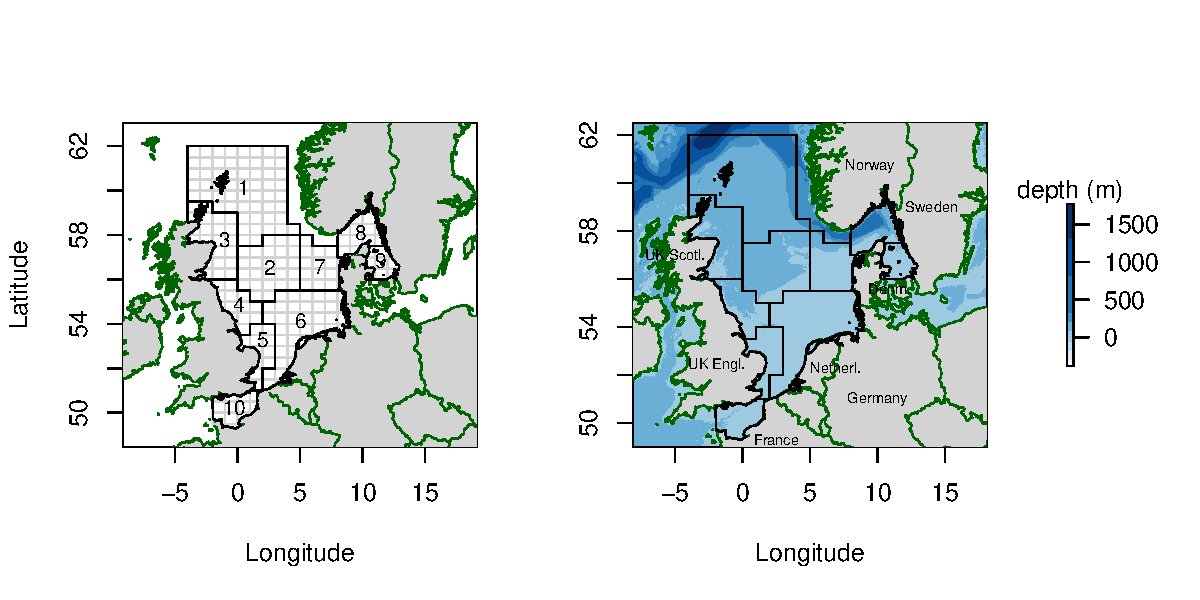
\includegraphics[width=0.95\textwidth]{figures/Newsurveyarea}} & 
\end{tabular}
\caption[]{Standard roundfish areas (RFAs) used for roundfish since 1980 and for all standard species since 1991 (left panel). RFA 10 was added in 2009. The number 1, for example, indicates ICES RFA 1. The small grey rectangles in the left panel indicates the statistical rectangles of approximately $30 \times 30$ nautical miles (these vary from ~28 nm wide in the north, to ~40 nm wide in the south of North sea) ($1^{o} \  \mathrm{Longitude} \ \times  \  0.5^{o} \ \mathrm{Latitude}$). \ed{include only left panel plot and reference our paper}.}
\label{icesroufismap}
\end{figure*} 

%In the North Sea International Bottom Trawl Surveys, trawl hauls are standardized by tow duration. A typical haul duration is 30 minutes, however, trawl hauls of 15-34 minutes are considered valid  \citep{ICES2015}. Accordingly, nations can reduce tow durations to 15 minutes when necessary and such reduction in tow times should not be interpreted as indication of reduced tow quality \citep{ICES2016Report}. In this section we propose a multinomial spatial ALK estimator \ref{sec:spatialModelALK}), and we also consider the spatial ALK model approach using continuation ratio logits proposed by \citet{berg2012spatial} (Section \ref{sec:BergModel}). We also give the estimators of abundance indices in Section \ref{sec:cpueestimators}.


\subsection{\large Multinomial spatial ALK  estimator}
\label{sec:spatialModelALK}
We assume a multinomial logistic model for proportion at age. Using such a model enables us to obtain smooth structures in the distribution of age given length. It also allows us to utilize spatial latent effects. Assume a fish can be of age $a = M,...,A$ where $M$ is the youngest age, and $A$ is the oldest age which is typically defined as a "plus group". In our application we define two ages as the reference ages, allowing for a reduction in the number of linear predictors and reducing modelling complexity issues such as convergence. This reduction of parameters is accomplished by assuming there exists a length $l^*$, such that all fish longer than $l^*$ are above age $M$, and all fish shorter than $l^*$ are below age $A$. Let $p_a(l,s)$ be the probability of a fish with length $l$ at location ${\bf s}$ to be of age $a$. That is,
\begin{equation}
p_a(l,s) = \frac{\exp(\mu_a({\bf s},l))}{1+ \sum_{i = M+1}^{A-1} \exp(\mu_i({\bf s},l))} \vspace{ 4mm} \ \ \ \text{for } a =M+1,...,A-1.
\end{equation}
Note that either $p_{A}(l,{\bf s})$ or $p_{M}(l,{\bf s})$ is known to be equal to zero, and the other is selected such that $\sum_a p_a = 1$, and where

\begin{equation}\label{eq:linearPred}
\mu_a({\bf s},l) = f_a(l) + \gamma_a({\bf s}) \vspace{ 4mm} \ \ \ \text{for } a =M+1,...,A-1.
\end{equation}
Here, $ f_a(l)$ is a continuous function of length and $\pmb{\gamma}$ is a mean zero Gaussian spatial random field with Mat\'{e}rn covariance function \citep{stein2012interpolation}. The spline $f_a (l)$ accounts for the fact that longer fish are typically older, and the spatial random field, $\pmb{\gamma}$, is intended to account for spatial variation in the ALK. The continuous function $f_a(l)$ in (\ref{eq:linearPred}) is modelled with usage of P-splines \citep{wood2017generalized}, and these spline regression coefficients are included as a mean zero Gaussian random effect. The precision matrix for the spline regression coefficients is constructed such that wiggliness is penalized, see \citet[page 239]{wood2017generalized} for details. The $\R$ package $\mgcv$ \citep{wood2015package} is used for extracting the precision matrix needed for the spline regression coefficients. The marginal variance of the P-splines regression coefficients, $\sigma_f^2$, is estimated in our inference procedure. We assume that the spatially Gaussian random field in (\ref{eq:linearPred}), $\pmb{\gamma}$, follows a stationary Mat\'{e}rn covariance structure defined as
\begin{equation}\label{eq:matern}
 \text{Cov}(\gamma(\mathbf{s}_1),\gamma(\mathbf{s}_2)) = \frac{\sigma^2_{\gamma}}{2^{\nu-1}\Gamma(\nu)}(\kappa||\mathbf{s}_1 -\mathbf{s}_2||)^{\nu}K_{\nu}(\kappa||\mathbf{s}_1-\mathbf{s}_2||),
\end{equation}
where $\sigma^2_{\gamma}$ is the marginal variance of the spatial field; $||\mathbf{s}_1-\mathbf{s}_2||$ is the distance between $\mathbf{s}_1$ and $\mathbf{s}_2$ in kilometres; $\kappa$ is a spatial scale parameter of the spatial field; $\nu$ is a smoothing parameter and $K_{\nu}(\cdot)$ is the modified Bessel function of the second kind with $\nu = 1$.  The spatial field is estimated with the stochastic partial differential equation (SPDE) procedure described in \citet{lindgren2011explicit}. The main concept behind the SPDE procedure is that the precision matrix of a spatial field with Mat\'{e}rn  covariance function can be approximated by a sparse matrix on a grid covering the area of interest. Such a grid and sparse precision matrix are constructed with use of the R-INLA package \citep{rue2009approximate}. The details regarding the construction of the mesh can be found at github (\href{https://github.com/OlavNikolaiBreivik/IBTSspatialALK}{https://github.com/OlavNikolaiBreivik/IBTSspatialALK}).

The constant $l^*$, which is included to reduce the number of parameters, is selected as the mid point between the shortest fish of age A and the longest fish of age M in the corresponding year and quarter.  A sensitivity analysis of this constant is performed by adjusting it up and down 5 cm for \ed{haddock} in year 2018 in Q1. 
%The point estimate of the $\text{mCPUE}_a$ then changed in the forth decimal, which we will consider negligible. 

%\clearpage
\begin{figure}[h!]
\begin{center}
\includegraphics[scale=0.5]{figures/mesh.jpeg}
 \caption{\ed{Mesh used in the case study for haddock in Section \ref{sec:data} for approximating (\ref{eq:matern}) with the SPDE-procedure. (update this plot for haddock)}}\label{fig:mesh}
\end{center}
\end{figure}
\noindent The ALK estimate is obtained by maximizing the likelihood. We maximize the likelihood with use of an R-Package {\sffamily TMB} \citep{kristensen2015tmb}, combined with the optimizing function {\sffamily nlminb} in R. In this application {\sffamily TMB} is advantageous as it uses Laplace approximation for the latent fields gaining computational efficiency, it also utilizes sparse structures in the latent fields, and uses automatic derivation. We define the spatial ALK model estimator as $\mathrm{ALK}_{a,l,h}^{M}$.


\subsubsection{Incorporating random haul effect (or haul-duration effects?)}
\label{sec:hauleffect}
We can extend the model in \ref{eq:linearPred} to include random effect of trawl hauls. Let  $h$ denote a trawl haul, then the linear predictor with random haul effect is defined as
\begin{equation}
\mu_{a}(a, \ l, \ h) = f_a(l) + \gamma_a({\bf s}) + \nu_{a} (h) \vspace{ 4mm} \ \ \ \text{for } a =M+1,...,A-1,
\label{eq:linearPredictorWithHaul}
\end{equation}
where $ f(\cdot)$ is a continuous function of length $l$; $\pmb{\gamma}$ is a mean zero Gaussian spatial random field with Mat\'{e}rn covariance function; and $\nu (\cdot)$ is an independent and identically distributed random haul effect. The parameter $\nu$ is intended to capture any haul variation, for example, a haul may encounter a school of fish of a certain age. This variation may 


\subsubsection{Incorporating the probability of mis-reading age}
\label{sec:misreading}

In this research, otoliths taken from a subsample of length-stratified data are used for age determination. These otolith structures  consist of periodic growth increments at the annual scale, which are used to determine the age of a fish. However, the process of estimating fish age can incorporate various sources errors, two of which are: 1) process error associated with structure being examined, and 2) error due to the element of subjectivity \citep{campana2001accuracy, hanselman2012statistical}. These errors can introduce considerable bias in estimates of population abundance \citep{bradford1991effects}. \citet{campana2001accuracy} describes process error as the incomplete growth sequence in the structure examined for a fish, which is typically biased towards under-ageing or over-ageing 

In this section, we extend equation.... to incorporate error of 
%\subsubsection{Variance estimation}
%The variance of the mCPUE can estimated directly from the model using the inverse of the negative Hessian matrix or bootstrapping


\subsection{\large Continuation ratio logits ALK estimator}
\label{sec:BergModel}
In this section we give the spatial ALK estimator developed by \citet{berg2012spatial} for estimating abundance at age indices. In this model, continuation ratio logits (CRLs) are used to model the distribution of ages, where generalized additive models (GAMs) are used for fitting these CRLs to model age as a smooth function of length and geographical position. GAMs elimnate the need of stratification for modelling regional differences in age-length structures. GAMs model the spatial effects as a smooth surface, predicting numbers-at-age at the haul level. 

Let the response variable be the age group of a fish, $a = M,...,A$, where $M$ denotes the youngest age category and $A$ is the oldest age category. Here $A$ is defined as a ``plus group'', which consists of fish of age $A$ or older. For each fish of age $a$, a set of covariates $\bf x$, which includes the length $l$ of the fish and the spatial coordinates of the fishery are known. The conditional probability of a fish being of age $a$ given that it is at least age $a$ is defined as 
\begin{equation}
\pi_{a} = P(Y = a \ | \ Y \ge a) = \frac{p_{a}}{p_{a} +...+ p_{A}},  \ \ \ a=M,..., A-1,
\label{eq:bergsprobability}
\end{equation}
and is accomplished through $A-M$ models. The set of continuation ratio logits are given in Generalized Additive Models (GAMs) of the form:
\begin{equation}
\mathrm{logit}(\pi_{a}  [{\bf x_{i}}]) = {\bf x_{i}^{*}} {\bf \theta_{a}} + f_{1a}(x_{1i}) + f_{2a}(x_{2i}, x_{3i}) + f_{3a}(x_{4i})x_{5i} +...,  \ \  \  a = M...A-1,
\label{eq:linearpredictorberg}
\end{equation}
where $\bf x_{i}$ is a vector of covariates, $\bf x_{i}^{*}$ is a subset of the covariates entering linearly in the model, $\bf \theta$ is the corresponding parameter vector, and $f_{j}$ is some smooth function of the covariates $x_{k}$, which may be one or more dimensions and also multiplied by known covariates. The estimated unconditional probabilities $\hat{p}_{a}$ can be calculated from the conditional probabilities $\hat{\pi}_{a}$ as follows:
\begin{equation}
\hat{p}_{M}  = \hat{\pi}_{M} 
\label{eq:unconditionalBerg1}
\end{equation}
\begin{align}
\hat{p}_{a} & = \hat{\pi}_{a} \left(1- \sum_{j=M}^{a-1} \hat{p}_{j} \right) = \hat{\pi}_{a} \prod_{j = M}^{a-1}  \left(1- \hat{\pi}_{j}  \right), \ \ \  a > M.
\label{eq:unconditionalBerg2}
\end{align}
In this model, a single reference age is defined. Also, there are $A-1$ linear predictor in this model, which can be interpreted as follows: the first linear predictor interprets the probability of the fish with age $M$. All other linear predictor interprets the probability of a fish of age $M+ j$ given that is it older than the fish of age in the previous age group, where $j=1,...,A-1$ \ed{(definition of older age group or plus group? above description about linear predictors needs verification and clarification)}. These GAMs are based on implementation in the  $\mgcv$ package for $\R$ by \citet{wood2015package}, where  thin plate regression splines with shrinkage smoothing are used for inputs \citep{berg2012spatial}.



\subsection{\large Estimators of age composition of fish}
\label{sec:cpueestimators}

In this research we use the estimators of abundance at age defined by ICES for the North Sea International Bottom Trawl Survey (Section \ref{sec:ICES-estimator}). These estimators are derived based on stratification by statistical rectangles and round fish areas (RFAs) \ed{(reference our paper here)}. \citet{berg2012spatial} proposed a simple estimator of abundance for application of the spatial ALK model developed in Section \ref{sec:BergModel}. This estimator is given in Section \ref{sec:BergIndex}.

\subsubsection{ICES-IBTS estimators}
\label{sec:ICES-estimator}
The estimators of abundance are haul-duration based and utilize an ALK approach. Catch per unit effort (CPUE) is defined as the number of fish of a certain species and age or length which are caught per hour trawl. In this section we define the CPUE mathematically, which explains how the index is calculated. For a given species of interest, let $n_{h,l}$ be the number of fish with length $l$ caught by trawl haul $h$. The CPUE for a given length $l$ by trawl haul $h$ is defined as 
\begin{equation}\label{eq:cpueHaul}
\mathrm{CPUE}_{h,l} =\frac{n_{h,l}}{d_h},
\end{equation}
were $d_h$ is the duration of the trawl in hours. The CPUE per age class is further defined as
\begin{equation}\label{eq:cpueALK}
\mathrm{CPUE}_{h,a} =\sum_{l \in {\bf L}}\mathrm{CPUE}_{h, l} \times ALK_{a,l,h}^{M},
\end{equation}
where ${\bf L}$ is the set of all length classes and $ALK_{a,l,h}$ is the age length key, which represents the estimated proportion of fish with age $a$ in $l$th length class in haul $h$. The mean CPUE per age in a statistical rectangle $s$ is further defined as
\begin{equation}\label{eq:cpueRec}
\mathrm{mCPUE}_{s,a} =\frac{\sum_{h \in H_{s}} \mathrm{CPUE}_{h,a}}{|H_{s}|}.
\end{equation}
Here $H_{s}$ represents the set of trawl hauls taken in statistical rectangle $s$, and $|H_{s}|$ is the number of hauls taken in the rectangle. The mCPUE in $p$th RFA is further defined as
\begin{equation}\label{eq:cpueRFA}
\mathrm{mCPUE}_{p,a} = \frac{ \sum_{s \in S_{p}} \mathrm{mCPUE}_{s,a}}{|S_{p}|} \omega_s,
\end{equation}
where $S_{p}$ is the set of all statistical rectangles in RFA $p$, $|S_{p}|$ is the number of statistical rectangles in RFA $p$, and $\omega_s$ is a weight factor for each statistical rectangle \citep{ICES2013}. For species such as saithe, herring, and sprat the indices at age are calculated using the mean over rectangles, weighted for the percentage of area with water depths between 10m-200m, and for RFAs 8 and 9 water depths between 10m-250m \citep{ICES2013}.

 The mean catch per unit at age in the whole study area is defined as
\begin{equation}
\text{mCPUE}_a= \frac{\sum_{p\in {\bf P}} A_{p}  \mathrm{mCPUE}_{p,a}}{A_{\text{total}}}.
\label{eq:abundanceestimatornorthsea}
\end{equation}
We refer to (\ref{eq:abundanceestimatornorthsea}) as the index of abundance at age, where ${\bf P}$ is the set of RFAs, $A_p$ is the area of RFA $p$, and $A_{\text{total}} = \sum_{p\in {\bf P}} A_{p}$ \ed{(see, our paper for details)}.
%mCPUE_{N,a} 

\subsubsection{\citet{berg2012spatial} estimator}
\label{sec:BergIndex}

\citet{berg2012spatial} define a simple estimator of abundance at age as
\begin{equation}
I_{ayq} = \frac{1}{h_{yq}} \sum_{i=1}^{n_{yq}}\hat{p}_{a} (\bf x_{i}),
\label{eq:bergIndex}
\end{equation}
where $I_{ayq}$ is the average predicted number of fish caught in age group $a$ per haul in year and quarter ($y,q$), $n$ is the total number of fish caught, $h$ is the number of hauls. The estimated unconditional probability, $\hat{p}_{a}$, of a fish being age $a$ is defined in equations \ref{eq:unconditionalBerg1} and \ref{eq:unconditionalBerg2}


\subsection{\large Variance estimation}
In \citet{berg2012spatial} bootstrapping is used to estimate uncertainties on the indices of abundance. In our approach, uncertainties on the indices are extracted \ed{from the inverse of negative Hessian matrix ....?}

%\clearpage
\section{RESULTS}
\label{sec:results}

The methods described in Section \ref{sec:methods} will be applied to eighteen years  (2001-2018) of data from the International bottom Trawl Survey obtained from the DATRAS database  (\href{https://datras.ices.dk}{https://datras.ices.dk}). The North Sea IBTS targets several demersal fish species (Table \ref{tab:otolithsTable} in Supplementary Materials \ref{secAp:otolithappendix}) but the focal species of this research is haddock.


\clearpage



\subsection{Comparison of spatial ALK estimators}

\clearpage
\subsection{Incorporating random haul effect}


\clearpage
\subsection{Incorporating probability of mis-reading age}



\clearpage
\section{DISCUSSION}
\label{sec:discussion}

\clearpage

%\subsection{North Sea haddock (\textit{Melanogrammus aeglefinus}) }
%\label{sec:data}
%The North Sea International Bottom Trawl Survey is an extensive survey dating back to 1991 with quarterly surveys in the winter months of February and March (Q1) and in the summer months of July-August (Q3). Research vessels from seven nations in the first quarter (Q1) and six nations in the third quarter (Q3) are used for conducting surveys on all finfish species (see Table \ref{countries} in Supplementary Materials \ref{secAp:areasfishedappendix} for participating nations). Several demersal fish species are targeted (Table \ref{tab:otolithsTable} in Supplementary Materials \ref{secAp:otolithappendix}) but the focal species of this research is haddock. Trawl hauls at each station are standardized by tow duration and the catches are subsampled in two stages to obtain biological data, such as individual fish length and weight, and to collect otoliths for age determination. These otoliths are collected from a length-stratified  subsample of fish measured for length
%Several demersal fish species are targeted (Table \ref{tab:otolithsTable} in Supplementary Materials \ref{secAp:otolithappendix})






\clearpage

\bibliographystyle{apalike}
\bibliography{BibliographyIbts}

\clearpage


\begin{center}
\textbf{\Large Supplemental Materials: Optimizing sampling effort of the North Sea International Bottom Trawl Survey.}
\end{center}
%%%%%%%%%% Merge with supplemental materials %%%%%%%%%%
%%%%%%%%%% Prefix a "S" to all equations, figures, tables and reset the counter %%%%%%%%%%
\setcounter{section}{0}
\setcounter{equation}{0}
\setcounter{figure}{0}
\setcounter{table}{0}
\setcounter{page}{1}
\makeatletter
\renewcommand{\thesection}{S\arabic{section}}
%\renewcommand{\theequation} {\arabic{section}. S\arabic{equation}}
%\renewcommand{\theequation}{S\arabic{equation}}
\renewcommand{\theequation}{S\arabic{section}.\arabic{equation}}
\renewcommand{\thefigure}{S\arabic{figure}}
\renewcommand{\bibnumfmt}[1]{[S#1]}
\renewcommand{\citenumfont}[1]{S#1}

\setcounter{table}{0}
\numberwithin{table}{section}
%\clearpage
\section{\large Areas fished by different countries in the North Sea IBTS}
\label{secAp:areasfishedappendix}
Typically, two different countries fish each rectangle so that at least two trawl hauls are made per rectangle, but intensified sampling is carried out in the following areas: at least 3 hauls per rectangle are taken in statistical rectangles  31F1, 31F2, 32F1, 33F4, 34F2, 34F3, 34F4, 35F3, 35F4; while six or more hauls per rectangle are taken in statistical rectangles  30F1, 32F2, 32F3, 33F2, 33F3 (ICES 1999).  The Skagerrak and Kattegat is fished solely by Sweden, who sample more than once in every rectangle while the west of Shetland (in Q1 and Q3) and inshore areas (Q3) is fished solely by Scotland. The edge of the Norwegian Trench is fished solely by Norway, but inshore areas near Denmark is fished by Denmark. The southern North Sea is fished by Denmark, Germany and England. France, typically, is the only country that surveys the western English Channel. Areas are surveyed by a single country because of the large proportion of untrawalable area (and subsequent gear damage issues experienced by other nations)  for efficient logistical purposes. Table \ref{countries} gives the countries and research vessels participating the North Sea IBTS.\\
\begin{small}
\begin{table}[h!]
\centering
\captionsetup{font=small, width = 15.5cm}{
\caption{Survey countries, vessel name, and period research vessels participating in first quarter (Q1) and third quarter (Q3) during 1997-2017.}\label{countries}}
\begin{tabular}{cccccccc}
\hline \\[0.1ex]
  & \multicolumn{2}{c}{\bf First Quarter (Q1)} & \multicolumn{2}{c}{\bf Third Quarter (Q3)}\\[1.5ex]
{\bf Country }  & Vessel name & Period    & Vessel name & Period  \\[0.5ex]
\hline \\[0.5ex]
Denmark  &   Dana   &   January-February  & Dana & July-August    \\[1ex]
France  & Thalassa II & January-February & - & -   \\[1ex]
Germany   &  Walther  Herwig III & January-February   &   Walther  Herwig III & July-August \\[1ex]
Netherlands &  Tridens 2 &  January-February   & - & -     \\[1ex]
Norway  &   G.O. Sars  & January-February &    Johan Hjort  & July   \\[1ex]
UK England &- & -&  Endeavour &  August-September  \\[1ex]
UK Scotland   &  Scotia III &  January-February & Scotia III &  July-August \\[1ex]
Sweden  &  Dana &  January-February  &  Dana &  August                  \\[0.5ex]
\hline
\end{tabular}
\end{table}
\end{small}




%\clearpage
\section{\large Otolith sampling per fish species}
\label{secAp:otolithappendix}
From 1991-2017, most countries conducted quota sampling of otoliths per length group in a RFA. But from 2013 Norway has been sampling one otolith per length class from each trawl haul (to 0.1$\cm$ below for shellfish, to 0.5$\cm$ below for herring and sprat and to 1$\cm$ below for all other species). From the first quarter in 2018 all countries are required to sample one otolith per length class per trawl haul.  Table \ref{tab:otolithsTable} gives the minimum sampling levels of otoliths for the target species. However, for the smallest size groups, that presumably contain only one age group, the number of otoliths per length class may be reduced, and more otoliths per length are required for the larger length classes.\\ %\\
\clearpage
\begin{small}
\begin{table}[h!]
\centering
\caption{Minimum sampling levels of otoliths by species for RFA or per trawl haul.}
\label{tab:otolithsTable}
\begin{tabularx}{\linewidth}{r l l l l X}
\toprule 
Period &  Species  & Minimum sampling levels of otoliths per length class    \\[0.7ex]
\midrule \\[0.1ex]
{\bf 1991-2017} & & {\bf Number of otoliths per length class in a RFA}  \\[1.0ex]
     & herring  &  $8$  otoliths per $\frac{1}{2}$ cm group \\[0.5ex]
     & sprat    & $16$  otoliths per $\frac{1}{2}$ cm length class  $8.0 -11.0$ cm\\[0.5ex]
              & & $12$  otoliths per $\frac{1}{2}$ cm length class  $\geq 11.0$ cm\\[0.5ex]
& mackerel      & $8$  otoliths per $\frac{1}{2}$ cm length class \\[0.5ex]
& cod       	  & $8$  otoliths per $1$ cm length class\\[0.5ex]
&haddock   	  & $8$  otoliths per $1$ cm length class \\[0.5ex]
&whiting    	  & $8$  otoliths per $1$ cm length class \\[0.5ex]
&Norway pout   & $8$  otoliths per $1$ cm length class\\[0.5ex]
&saithe        & $8$  otoliths per $1$ cm length class \\[1ex] 
& All target species      &  From 2013 Norway and Scotland, and  Netherlands from 2016 \\[0.7ex] 
&& have been sampling 1 otolith per length class from each trawl haul \\[0.7ex] 
&& (to 0.1$\cm$ below for shellfish, to 0.5$\cm$ below for herring and sprat, and \\ [0.7ex] 
&& to 1$\cm$ below for all other species).\\[1.7ex] 

{\bf 2018} & & {\bf Number of otoliths per length class per trawl haul}  \\[1.0ex]
  & herring  &  $1$  otolith per $\frac{1}{2}$ cm group \\[0.5ex]
     & sprat    & $1$  otolith per $\frac{1}{2}$ cm length class  $8.0 -11.0$ cm\\[0.5ex]
              & & $1$  otolith per $\frac{1}{2}$ cm length class  $\geq 11.0$ cm\\[0.5ex]
& mackerel      & $1$  otolith per $1$ cm length class \\[0.5ex]
& cod       	  & $1$  otolith per $1$ cm length class\\[0.5ex]
& haddock & $2$  otoliths per $5$ cm length class $11 -15, \ 16-20, \ 21-25, \ 26-30$ cm \\[0.5ex]
& Norway pout & $2$  otoliths per $5$ cm length class $5 -10, \ 11-15$ cm\\[0.5ex]
               & & $2$  otoliths per $1$ cm length class $> 15$ cm\\[1.0ex]
&saithe        & $1$  otolith per $1$ cm length class \\[0.5ex]  
&plaice       & $1$  otolith per $1$ cm length class \\[0.1ex]
\bottomrule         
\end{tabularx}
\end{table}
\end{small}


 
\end{document}